\documentclass[final]{beamer}
\usepackage{algorithmic}
\usepackage{algorithm}
\usepackage[orientation=portrait,
		size=custom, width=55.8, height=91.4,  % poster size 22in=55.88cm 91.44cm=36in
		scale=.99
	]{beamerposter}
\usepackage{listings}
\usepackage[american]{babel}  % language 
\usepackage[utf8]{inputenc}   % std linux encoding

\usetheme{pgassc11poster}            % our poster style
%--set colors for blocks (without frame)---------------------------------------
\setbeamercolor{block title}{fg=ngreen,bg=white}
\setbeamercolor{block body}{fg=black,bg=white}
%--set colors for alerted blocks (with frame)----------------------------------
%--textcolor = fg, backgroundcolor = bg, dblue is the jacobs blue
\setbeamercolor{block alerted title}{fg=white,bg=dblue}%frame color
\setbeamercolor{block alerted body}{fg=black,bg=dblue!10}%body color

%==Titel, date and authors of the poster=======================================
\title{Alternative High Performance Benchmarks in UPC}
\author{Kurt Rudolph, Vivek Kale, Lawrence C. Angrave, William D. Gropp}
\institute{Department of Computer Science, University of Illinois Urbana-Champaign}
\date{\today}
%
%==some usefull qm commands====================================================
%  |x>
\newcommand{\ket}[1]{\left\vert#1\right\rangle}
%  <x|
\newcommand{\bra}[1]{\left\langle#1\right\vert}
%  <x|y>
\newcommand{\braket}[2]{\left< #1 \vphantom{#2}\, \right\vert\left.\!\vphantom{#1} #2 \right>}
%  <x|a|y>
\newcommand{\sandwich}[3]{\left< #1 \vphantom{#2 #3} \right #2 \left|\vphantom{#1 #2} #3 \right>}
%  d/dt
\newcommand{\ddt}{\frac{d}{dt}}
%  D/Dx
\newcommand{\pdd}[1]{\frac{\partial}{\partial#1}}
%  |x|
\newcommand{\abs}[1]{\left\vert#1\right\vert}
%  k_{x}
\newcommand{\kv}[1]{\mathbf{k}_{#1}}




\begin{document}
	\begin{frame}[t]
		\begin{columns}[t] 
			  \begin{column}{0.60\paperwidth} 
%=======================Avstract======================================================================================
				\begin{alertblock}{Abstract}
					Benchmarks for High-Performance clusters generally focus on floating-point intensive calculations.  Few of these address data intensive graph operations, a class of computation rapidly growing in demand. As an alternative to standard floating-point benchmarks, a new benchmark, the Graph 500 has been proposed. The benchmark employs multiple implementations in MPI and MPI-RMA. However, a PGAS model has yet to be developed. This project focuses on understanding what capabilities a UPC Graph 500 implementation may offer. Specifically, this is done through: 1. the UPC expressibility for irregular graph operations seen in Graph 500 and 2. performance testing of the efficiency of UPC in the context of irregular parallelism.
				\end{alertblock}
				\vskip2ex
%=======================Linked List Traversal======================================================================================
				\begin{block}{Linked List Traversal}
					As a simple test to measure the efficiency of UPC when performing graph operations, various linked
list structure have been built and a traversal mesuring clock cycles is taken for each. The affinity of
the nodes are distributed across all processes in the group and colored according. Successive nodes
in linked list are allocate successively and have afinity according process and a single UPC process traverses the linked list.
				\vskip1ex
				\setbeamercolor{block title}{fg=dgreen,bg=white}
				\setbeamercolor{block body}{fg=black,bg=white}
				\begin{columns}[t,totalwidth=0.60\paperwidth]
					\begin{column}{0.28\paperwidth}
						\setbeamercolor{block alerted title}{fg=white,bg=dgreen}%frame color
						\setbeamercolor{block alerted body}{fg=black,bg=dgreen!10}%body color
						\begin{alertblock}{\small Test Info}
							\begin{itemize}
								\item 32 IBM Power7 Cores
								\item 32 UPC Processes per run
								\item 32 to 3768 traversal nodes incrimenting by 32 per run
								\item Each run repeated 8 times 
							\end{itemize}
						\end{alertblock}
					\end{column}
					\begin{column}{0.28\paperwidth}
						\vskip2ex
						\begin{block}{\small Sequential Process, Sequential Node\vskip2ex}
							\begin{columns}[t,totalwidth=0.28\paperwidth]
								\begin{column}{0.10\paperwidth}
									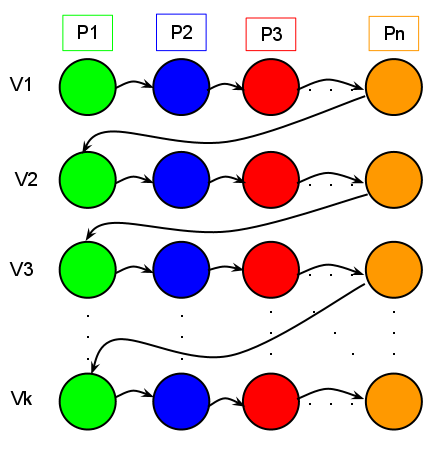
\includegraphics[width=0.12\paperwidth]{img/linked_list/seq_proc_seq_node}
								\end{column}
								\begin{column}{0.14\paperwidth}
									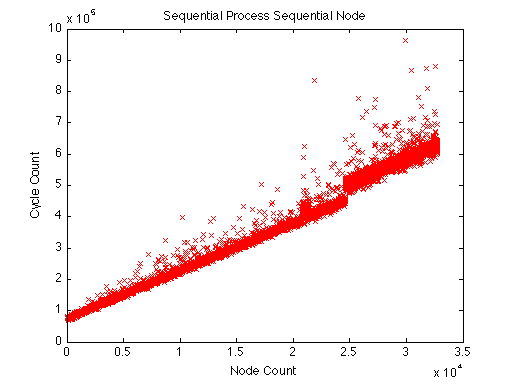
\includegraphics[width=0.16\paperwidth]{img/data/seq_proc_seq_node}
								\end{column}
							\end{columns}
						\end{block}
					\end{column}
				\end{columns}
				\vskip2ex
				\begin{columns}[t,totalwidth=0.60\paperwidth]
					\begin{column}{0.28\paperwidth}
						\begin{block}{\small Sequential Node, Sequential Process\vskip2ex}
							\begin{columns}[t,totalwidth=0.28\paperwidth]
								\begin{column}{0.10\paperwidth}
									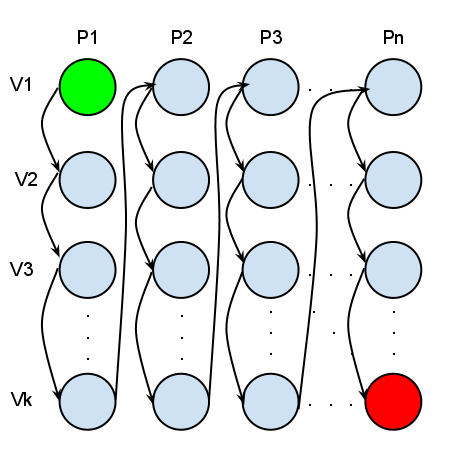
\includegraphics[width=0.12\paperwidth]{img/linked_list/seq_node_seq_proc}
								\end{column}
								\begin{column}{0.14\paperwidth}
									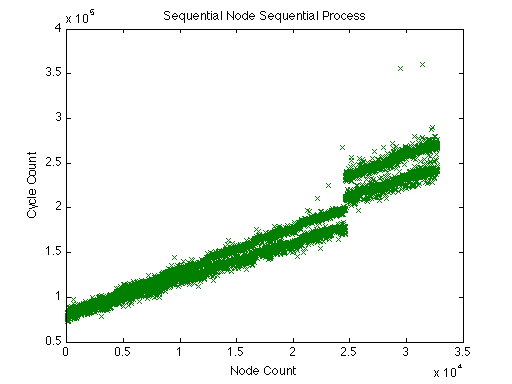
\includegraphics[width=0.16\paperwidth]{img/data/seq_node_seq_proc}
								\end{column}
							\end{columns}
						\end{block}
					\end{column}
					\begin{column}{0.28\paperwidth}
						\begin{block}{\small Random Process, Random Node\vskip2ex}
							\begin{columns}[t,totalwidth=0.28\paperwidth]
								\begin{column}{0.10\paperwidth}
									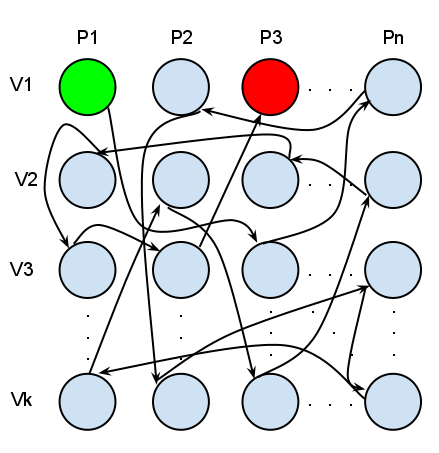
\includegraphics[width=0.12\paperwidth]{img/linked_list/rand_proc_rand_node}
								\end{column}
								\begin{column}{0.14\paperwidth}
									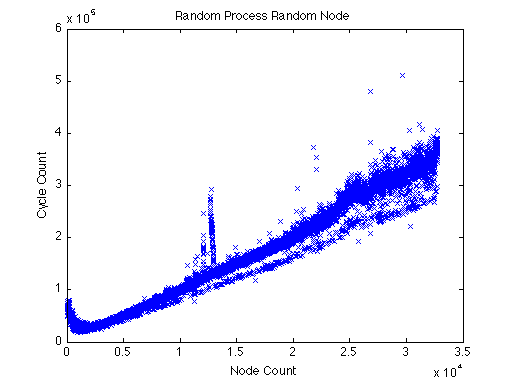
\includegraphics[width=0.16\paperwidth]{img/data/rand_proc_rand_node}
								\end{column}
							\end{columns}
						\end{block}
					\end{column}
				\end{columns}
				\vskip3ex
				\begin{columns}[t,totalwidth=0.60\paperwidth]
					\begin{column}{0.28\paperwidth}
						\begin{block}{\small Cumulative Results\vskip2ex}
							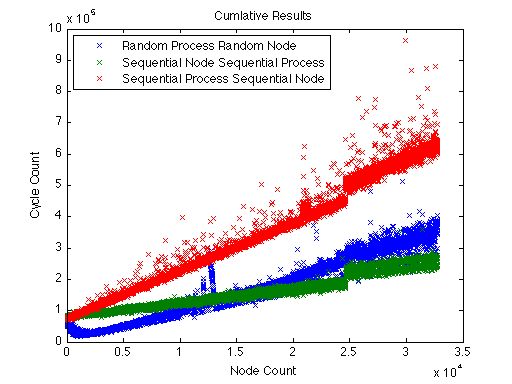
\includegraphics[width=0.28\paperwidth]{img/data/cumlative_traversal}
						\end{block}
					\end{column}
					\begin{column}{0.28\paperwidth}
						\setbeamercolor{block title}{fg=red,bg=white}
						\setbeamercolor{block body}{fg=black,bg=white}
						\begin{block}{\small Discussion\vskip2ex}
							The results give insight into how UPC graph operations may perform on the system.  Having a single process performing the linked list traversal provides a baseline for a fully optimized for parallel graph algorithm.  

							The jump at 2600 nodes indicates the amount of data required to perform the traversal has overflowed the capacity of the CPUs cache's.  After that point much slower access to disk must be performed in order to complete the computation.   
						\end{block}
					\end{column}
				\end{columns}
				\end{block}
				\vskip2ex
%=======================Random Access======================================================================================
				\begin{block}{Parallel Random Access}
					When performing graph operations, random access to memory and random process communication
are generally very common. This test looks at how well a UPC Graph 500 implementation may
handle these operations in parallel. To do so, we implement a dot product employing randomized
access and communication through the RDMA. The affinity to the vectors are distributed across
all processes in the group and colored accordingly. Successive vector positions are stored successive
memory locations of the according process. Accesses are performed simultaneously by all 32 UPC
threads. The test is set in the same manor as the proceeding; 32 IBM Power7 cores, 32 UPC processes per run, 32 to 3768 memory accesses and array elements per process per run, and each run is repeated 8 times.   
				\end{block}
				\begin{columns}[t,totalwidth=0.60\paperwidth]
					\begin{column}{0.26\paperwidth}
						{\small \lstinputlisting[language=C, basicstyle=\footnotesize]{ code_sample/upcRandomAccess.c}}
					\end{column}
					\begin{column}{0.10\paperwidth}
						\begin{columns}[t,totalwidth=0.10\paperwidth]
							\begin{column}{0.10\paperwidth}
								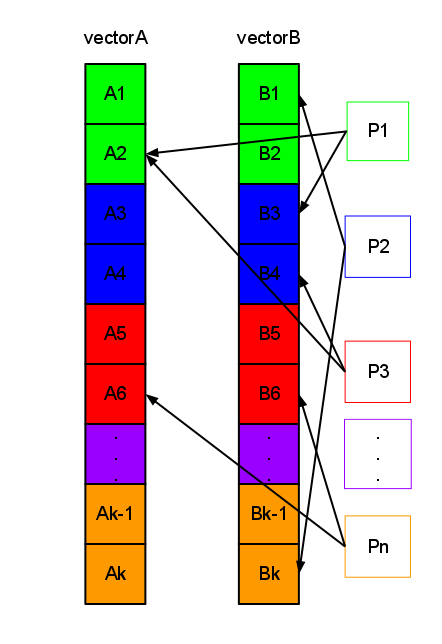
\includegraphics[width=0.09\paperwidth]{img/rand_access}
							\end{column}
						\end{columns}
					\end{column}
					\begin{column}{0.24\paperwidth}
						\begin{columns}[t,totalwidth=0.22\paperwidth]
							\begin{column}{0.24\paperwidth}
								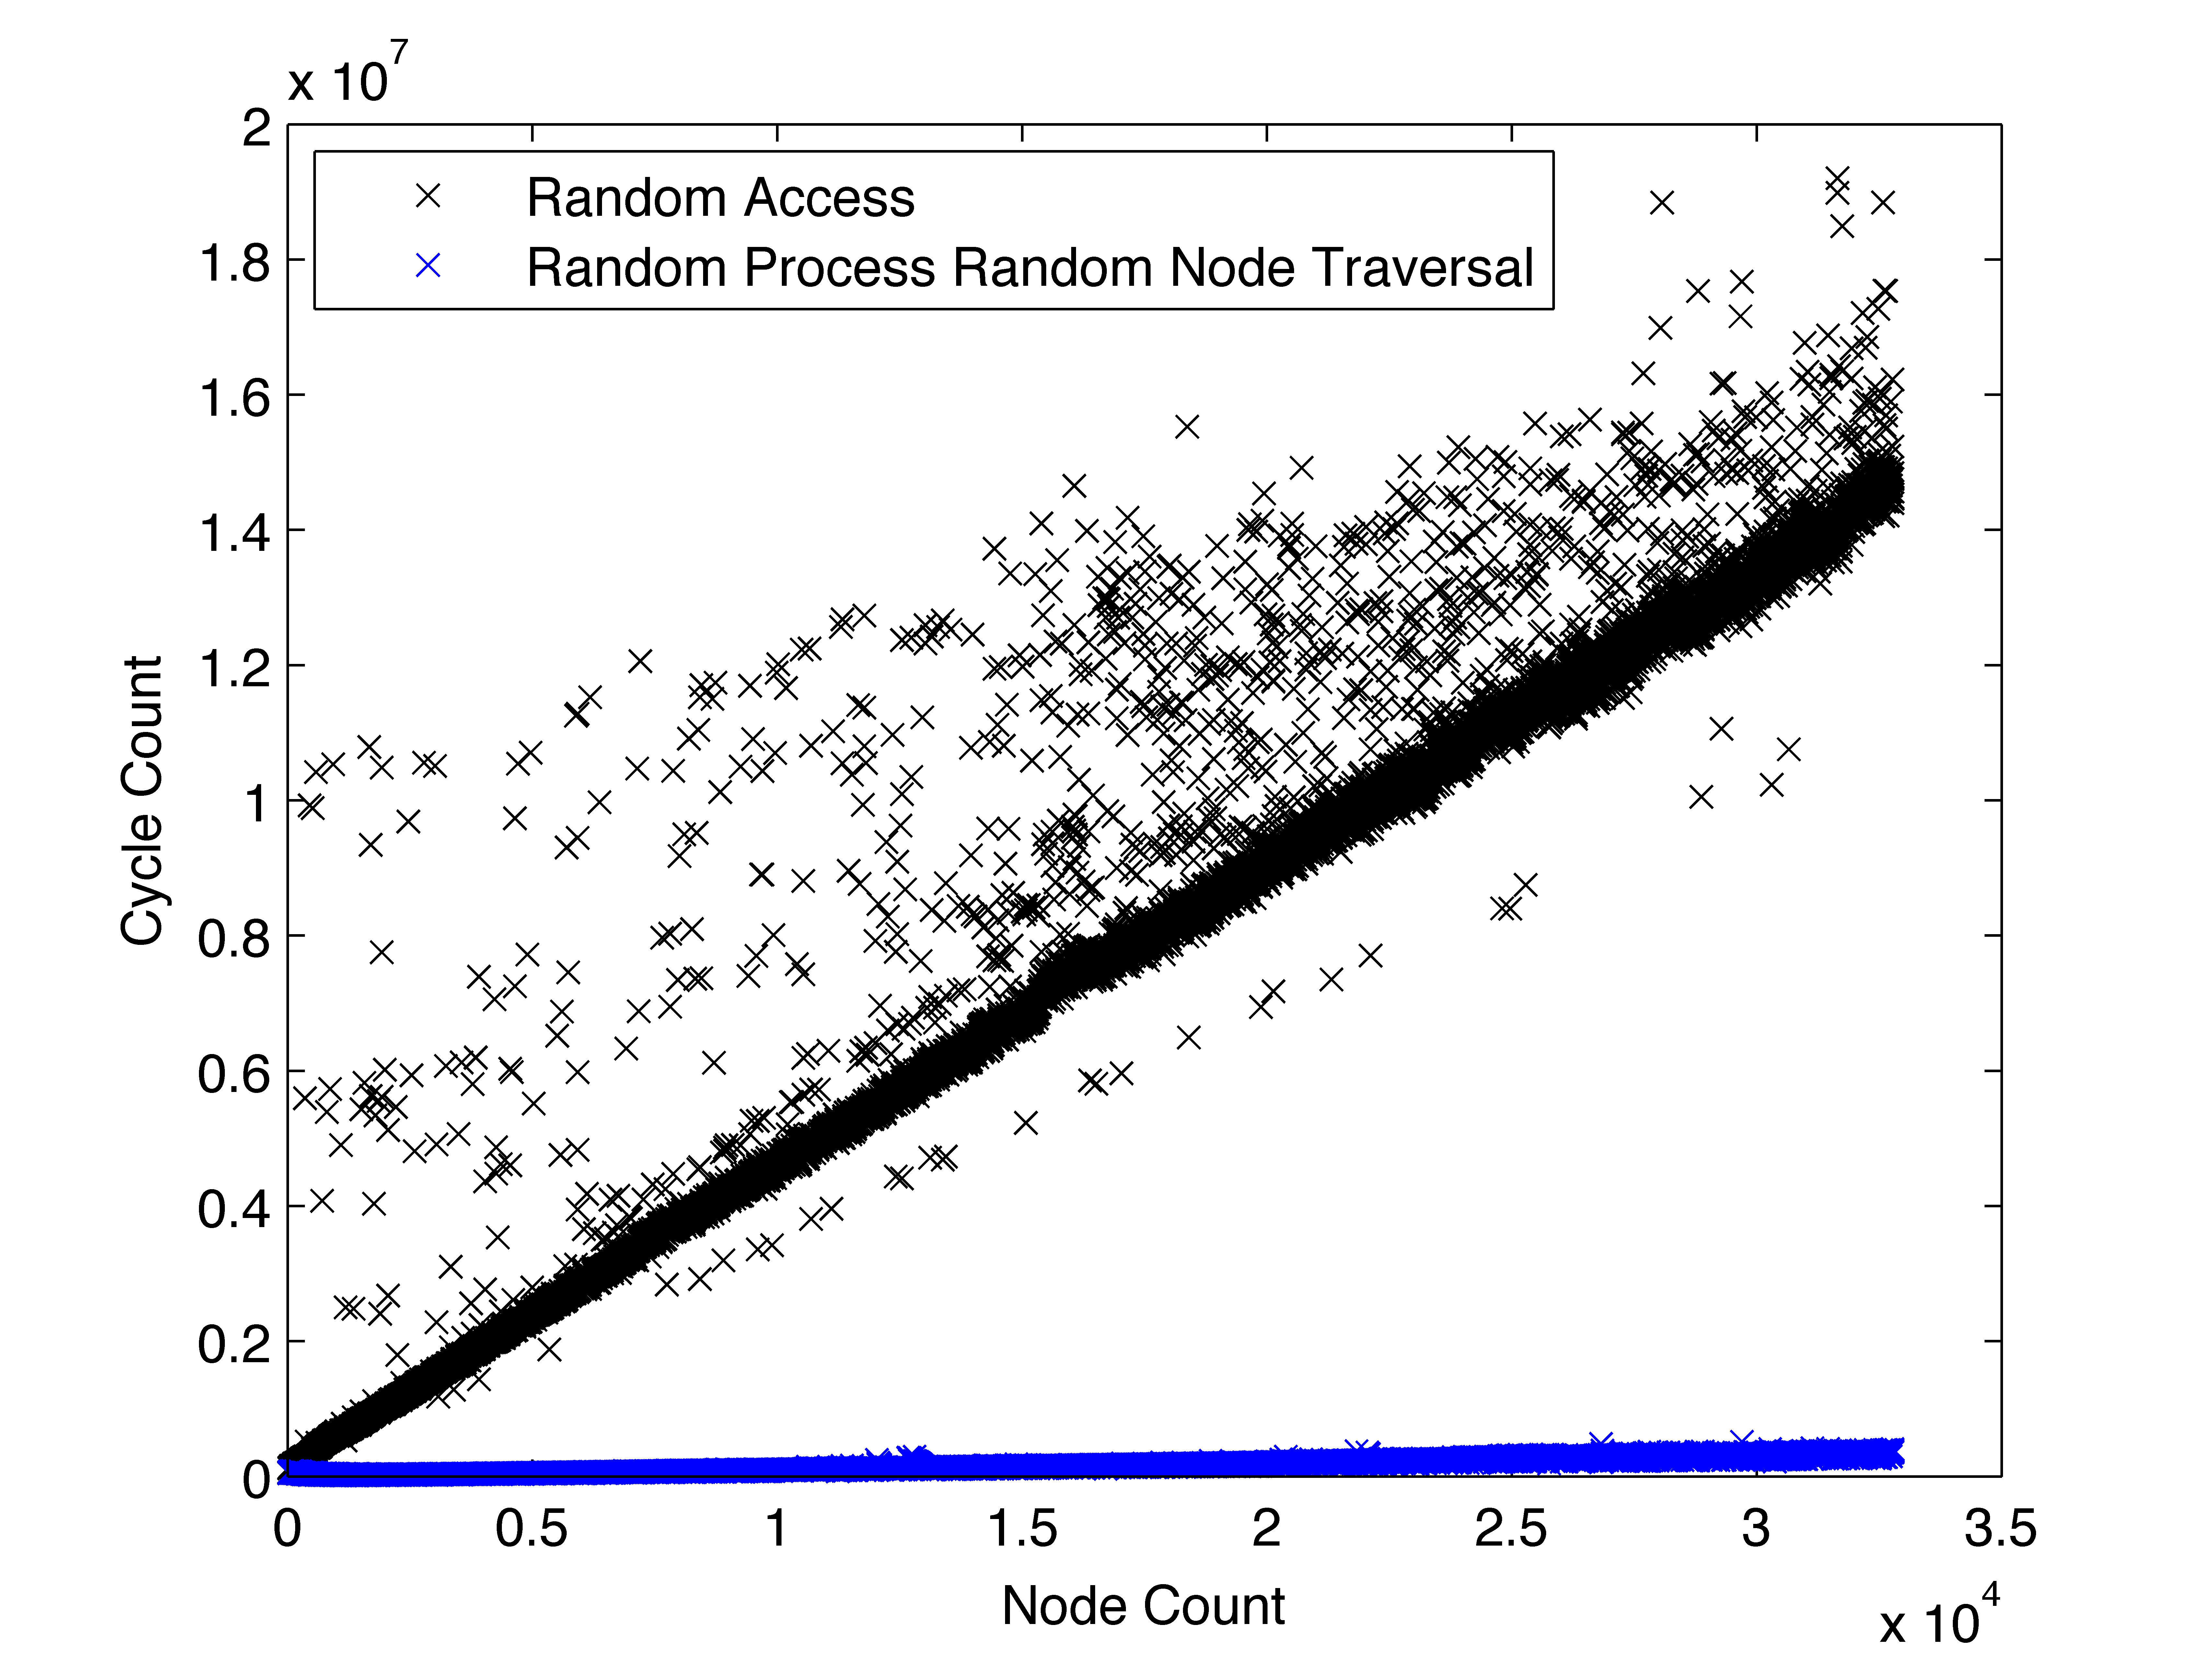
\includegraphics[width=0.26\paperwidth]{img/data/random_access}
							\end{column}
						\end{columns}
					\end{column}
				\end{columns}
				\vskip1ex
%=======================Multi Process Linked List Traversal======================================================================================
			\end{column}
			\begin{column}{0.28\paperwidth}
%=======================Discussion=======================================================================================================
				\begin{block}{Graph 500 BFS}
					Currently, the Graph 500 employs multiple implementations using MPI and OpenMP.  
					
					The "Simple" MPI implementation achieves two-sided communication through communicator functions such as  \emph{send} and \emph{receive}. Sample from Graph500 BFS MPI Simple:\vspace{2 mm}
					\lstinputlisting[language=C, basicstyle=\footnotesize]{ code_sample/mpiSimpleSample.c}
					 \vspace{5 mm}
					  The "One Sided" MPI implementation achieves one-sided communication through MPI \emph{windows}, a feature built into MPICH2 API.  When a thread creates an MPI \emph{window} access to another threads address space is enabled through the variables associated through that window.  Sample from the Graph500 BFS MPI One Sided: 
					  \vspace{2 mm}
					  \lstinputlisting[language=C, basicstyle=\footnotesize]{ code_sample/mpiOneSidedSample.c} 
					  \vspace{5 mm}
					  A UPC implementation of the Graph 500 will not require "windows" to achieve one sided communication.  However, address space used in any collective operations need to be allocated in shared memory space and receive the according performance loss of accessing memory via a shared pointer over a local pointer.  MPI collectives from the Graph500 BFS implemented in UPC take the simpler implementation as follows: 
					  \vspace{2 mm}
					  \lstinputlisting[language=C, basicstyle=\footnotesize]{ code_sample/upcOneSidedSample.c} 
				\end{block}
%=======================Conclusion========================================================================================================
				\begin{block}{Summary}
					The	\emph{Linked List Traversal} section attempts to emulate graph operations in UPC as simple as possible.  The purpose is to isolate the fundamental task (traversing a linked list) of any graph operation.

					The second section, \emph{Parallel Random Access}, attempts emulate a fully parallel graph operation in UPC.  The purpose is to identify how well UPC performs massively parallel graph operations with memory affinity randomly distributed to each of the processes.  
			
					The Proceeding section, \emph{Graph 500 BFS}, attempts to compare the current MPI and MPI-RMA implementations of the current Graph 500 to a potential UPC implementation.
				\end{block}
%=======================References========================================================================================================
				\begin{block}{References}
					\begin{thebibliography}{7}
						{\tiny
						\bibitem{hpcs_graph_benchmark}
							\emph{Design and Implementation of the HPCS Graph Analysis Benchmark
on Symmetric Multiprocessors}. D.A. Bader, M. Parashar, S. Varadarajan, and V.K. Prasanna, editors, Proc. 12th Int'l. Conf. on High Performance Computing (HiPC 2005), volume 3769 of LNCS, pages 465--476, Goa, India, December 2005. Springer.
							\url{http://www.cse.psu.edu/~madduri/papers/SSCA2-HiPC05.pdf}
						\bibitem{Introduction_To_UPC}
							\emph{Introduction to UPC and Language Specification}
							W. Carlson, J. Draper, D. Culler, K. Yelick, E. Brooks, and K. Warren. CCS-TR-99-157, IDA Center for Computing Sciences, 1999.
						  \url{http://upc.lbl.gov/publications/UPC-TR-Original99.pdf}
						\bibitem{UPC_Language_Spcification}
							\emph{A publication of the UPC Consortium}
							UPC Consortium, the current release of the UPC Language Specification is version 1.2, finalized in June of 2005.
							\url{http://upc.gwu.edu/docs/upc_specs_1.2.pdf}
						\bibitem{MPI}
							\emph{MPI: A Message-Passing Interface Standard} Message Passign Interface Forum, Version 2.2, September 4, 2009 
							\url{http://mpi-forum.org/docs/mpi-2.2/mpi22-report.pdf}
						\bibitem{MPI}
						}
					\end{thebibliography}
				\end{block}
			\end{column}
		\end{columns}
	\end{frame}
\end{document}




%--set custom colors---------------------------------------------------------------
 %  \setbeamercolor{block alerted title}{fg=black,bg=gray!50}%frame color
%   \setbeamercolor{block alerted body}{fg=black,bg=gray!30}%body color
